\section{Measuring analog voltages}

The main part of the data collection process is the PR2040 Microcontroller, which has built-in Analog-to-Digital Converters (ADCs). These ADCs convert electronic voltages ranging from Ground ($\SI{0}{V}$) to a reference voltage $U_{ref}$ into digital numbers, with a resolution set to 12 bits. This means the digital result from an ADC falls between $0$ and $2^{12} = 4096$. In theory this mapping should be proportional but in practise there are small uncertainties in this conversion process due to the resolution, as depicted in \cref{fig:ADC-Curve}. This figure shows that the uncertainty of a value acquired by an ADC is half the voltage corresponding to the least significant bit (LSB), which can be calculated as:

\begin{equation*}
	\sigma = \pm{} U_{ref} \cdot \frac{1}{2} \cdot \frac{1}{2^{resolution}} = \pm{} U_{ref} \cdot 2^{-(resolution + 1)}\,.
\end{equation*}

\begin{figure}[htb]
		\centering
		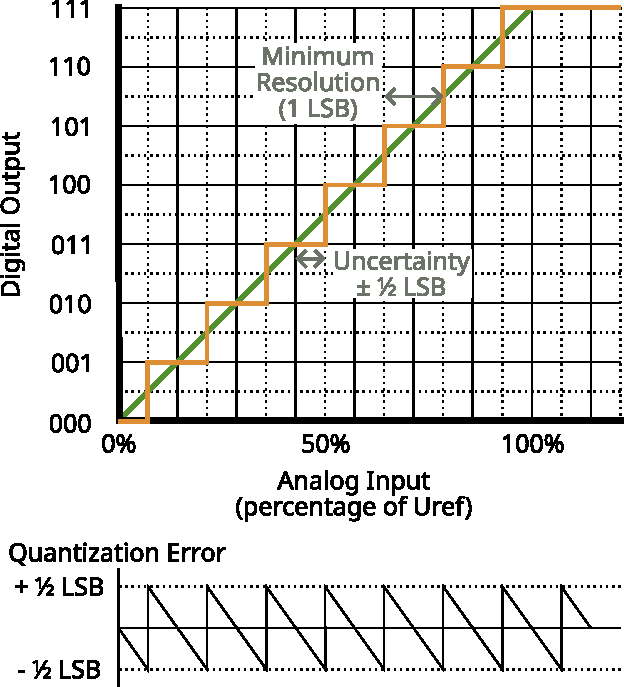
\includegraphics[width=0.6\textwidth]{./fig/ADC-conversion-curve-export.pdf}
		\caption{Conversion from an analog voltage do a digital number with an ADC}
		\label{fig:ADC-Curve}
\end{figure}

In practice, there are further reasons for short-term fluctuations in voltage which are bigger than the quantization uncertainty. Therefore, the proper uncertainty of an ADC in an electronic application can be determined through a  calibration process. A detailed explanation and characterisation of the Raspberry Pi Picos ADCs is available on \href{http://pico-adc.markomo.me/}{this website}.

The \href{https://datasheets.raspberrypi.com/rp2040/rp2040-datasheet.pdf}{data sheet} explains that four ADC channels (ADC0 to ADC3) are connected to GPIO Pins and the fifth ADC channel (ADC4) is connected to an internal temperature sensor. Notably the fourth channel ADC3 is connected to an onboard attenuator. This configuration is intended to be used to measure the VSYS voltage of the Raspberry Pi Pico board.

Each channel is linked to a single Analog-to-Digital Converter (ADC) through an internal switch, allowing the selection of one channel at a time. The shared ADC operates with a maximum sampling rate of 500 kilosamples per second (KSps). This sampling rate can be utilized for measuring voltages on a single channel at the full sampling speed (simplex). Alternatively, it can simultaneously measure two channels by periodically switching between them, effectively halving the sampling rate to 250 KSps per channel. The level of accuracy and sampling rate is sufficient for using the system as the core of a simple oscilloscope which periodically acquires ADC values and streams the data to another device for further processing.

An ADC can only measure voltages between $\SI{0}{V}$ and $U_{ref}$ but we aim to build an oscilloscope capable of measuring both positive and negative voltages within a range, for instance, $\vert U \vert > \SI{10}{V}$. To achieve this, an analog front-end is needed to map voltages from $-U_{max}$ to $+U_{max}$ into an analog voltage suitable for the ADC. Furthermore the input voltage range should be adjustable and there should be an over-voltage protection on the signal inputs. This allows for the measurement of higher voltages with less precision or lower voltages with higher precision.
